%******************************************************** -*-LaTeX-*- ******************************
%                                                                                                  *
% v3.0.2.0.2 Relationen und Funktionen - Geometrisches Bild.tex                                    *
%                                                                                                  *
% Copyright (C) 2023 Kategory GmbH \& Co. KG (joerg.kunze@kategory.de)                             *
%                                                                                                  *
% v3.0.2.0.2 Relationen und Funktionen - Geometrisches Bild is part of kategoryMathematik.         *
%                                                                                                  *
% kategoryMathematik is free software: you can redistribute it and/or modify                       *
% it under the terms of the GNU General Public License as published by                             *
% the Free Software Foundation, either version 3 of the License, or                                *
% (at your option) any later version.                                                              *
%                                                                                                  *
% kategoryMathematik is distributed in the hope that it will be useful,                            *
% but WITHOUT ANY WARRANTY; without even the implied warranty of                                   *
% MERCHANTABILITY or FITNESS FOR A PARTICULAR PURPOSE.  See the                                    *
% GNU General Public License for more details.                                                     *
%                                                                                                  *
% You should have received a copy of the GNU General Public License                                *
% along with this program.  If not, see <http://www.gnu.org/licenses/>.                            *
%                                                                                                  *
%***************************************************************************************************

\documentclass[a4paper]{amsart}
% \documentclass[a4paper]{book}

%-----------------------------------------------------------------------------------------------------*
% package:                                                                                            *
%-----------------------------------------------------------------------------------------------------*
\usepackage{amssymb}
\usepackage{amsfonts}
\usepackage{amsmath}
\usepackage{amsthm}

\usepackage{mathabx}

\usepackage{a4wide} % a little bit smaller margins

\usepackage{graphicx}
\usepackage{hyperref}
\usepackage{algorithmic}
\usepackage{listings}
\usepackage{color}
\usepackage{colortbl}
\usepackage{sidecap}
\usepackage{comment}
\usepackage{tcolorbox}
\usepackage{collect}

\usepackage{upgreek}

% \usepackage{diagrams}

\usepackage[german]{babel}
\usepackage[none]{hyphenat}
\emergencystretch=4em

\usepackage[utf8]{inputenc} % to be able to use äöü as characters in text
\usepackage[T1]{fontenc} % to be able to use äöü in lables
\usepackage{lmodern}     % to avoid pixelation introduced by fontenc

\usepackage{hyperref}

\usepackage{tikz}
\usepackage{tikz-cd}
\usetikzlibrary{babel}

%-----------------------------------------------------------------------------------------------------*
% theorem:                                                                                            *
%-----------------------------------------------------------------------------------------------------*
\theoremstyle{definition}
\newtheorem{theorem}{Theorem}[subsection]

\newcommand{\myTheorem}[1]{%
  \newtheorem{jk#1}[theorem]{#1}
  \newenvironment{#1}[1]{%
    \expandafter\begin{jk#1} \expandafter\label{#1:##1}\textbf{(##1):}
  }{%
    \expandafter\end{jk#1}
  }
}

\myTheorem{Definition}
\myTheorem{Proposition}
\myTheorem{Theorem}
\myTheorem{Example}
\myTheorem{Remark}

\definecollection{jkjkFrage}
\newtheorem{jkFrage}[theorem]{Frage}
\newenvironment{Frage}[1]{%
  \expandafter\begin{jkFrage} \expandafter\label{Frage:#1}\textbf{(#1):}
  \begin{collect}{jkjkFrage}{}{}
    \item \ref{Frage:#1} #1
  \end{collect}
}{%
  \expandafter\end{jkFrage}
}

\newcommand{\myRef}[2]{[#1 \ref{#1:#2}, ``#2'']}

\renewcommand{\proofname}{Beweis}

%-----------------------------------------------------------------------------------------------------*
% operator:                                                                                           *
%-----------------------------------------------------------------------------------------------------*
\DeclareMathOperator{\End}{End}
\DeclareMathOperator{\Ker}{Ker}
\DeclareMathOperator{\Mat}{Mat}
\DeclareMathOperator{\rank}{rank}
\DeclareMathOperator{\ggT}{ggT}
\DeclareMathOperator{\len}{len}
\DeclareMathOperator{\ord}{ord}
\DeclareMathOperator{\kgV}{kgV}
\DeclareMathOperator{\id}{id}
\DeclareMathOperator{\red}{red}
\DeclareMathOperator{\supp}{supp}
\DeclareMathOperator{\Bild}{Bild}
\DeclareMathOperator{\Rang}{Rang}
\DeclareMathOperator{\Det}{Det}
\DeclareMathOperator{\Hom}{Hom}

\DeclareMathOperator{\sub}{sub}
\DeclareMathOperator{\blk}{blk}
\DeclareMathOperator{\minimal}{minimal}
\DeclareMathOperator{\maximal}{maximal}

\definecolor{mygreen}{rgb}{0,0.6,0}
\definecolor{mygray}{rgb}{0.5,0.5,0.5}
\definecolor{mymauve}{rgb}{0.58,0,0.82}

\lstset{ %
  backgroundcolor=\color{white},   % choose the background color
  basicstyle=\ttfamily\footnotesize,        % size of fonts used for the code
  breaklines=true,                 % automatic line breaking only at whitespace
  captionpos=b,                    % sets the caption-position to bottom
  commentstyle=\color{mygreen},    % comment style
  escapeinside={\%*}{*)},          % if you want to add LaTeX within your code
  keywordstyle=\color{blue},       % keyword style
  stringstyle=\color{mymauve},     % string literal style
  frame=single
}

\setcounter{MaxMatrixCols}{20}

%******************************************************************************************************
%                                                                                                     *
% definition:                                                                                         *
%                                                                                                     *
%******************************************************************************************************
\newcommand{\R}{\ensuremath{\mathbb{ R }}}
\newcommand{\Q}{\ensuremath{\mathbb{ Q }}}
\newcommand{\Z}{\ensuremath{\mathbb{ Z }}}
\newcommand{\N}{\ensuremath{\mathbb{ N }}}
\newcommand{\C}{\ensuremath{\mathbb{ C }}}
\newcommand{\A}{\ensuremath{\mathbb{ A }}}
\newcommand{\F}{\ensuremath{\mathbb{ F }}}
\newcommand{\K}{\ensuremath{\mathbb{ K }}}
\newcommand{\Pb}{\ensuremath{\mathbb{ P }}}

\newcommand{\M}{\ensuremath{\mathcal{ M }}}
\newcommand{\V}{\ensuremath{\mathcal{ V }}}

\newcommand{\AAA}{\ensuremath{\mathcal{ A }}}
\newcommand{\BB}{\ensuremath{\mathcal{ B }}}
\newcommand{\CC}{\ensuremath{\mathcal{ C }}}
\newcommand{\EE}{\ensuremath{\mathcal{ E }}}
\newcommand{\KK}{\ensuremath{\mathcal{ K }}}
\newcommand{\MM}{\ensuremath{\mathcal{ M }}}
\newcommand{\PP}{\ensuremath{\mathcal{ P }}}
\newcommand{\ZZ}{\ensuremath{\mathcal{ Z }}}

\newcommand{\imporant}[1]{ \textcolor{red}{\textbf{#1}} }

\newcommand{\bb}[1]{\mathbf{#1}}
\newcommand{\balpha}{\boldsymbol{\upalpha}}
\newcommand{\bbeta}{\boldsymbol{\upbeta}}
\newcommand{\bgamma}{\boldsymbol{\upgamma}}
\newcommand{\bdelta}{\boldsymbol{\delta}}
\newcommand{\bmu}{\boldsymbol{\upmu}}

\newcommand{\z}[1]{\Z_{#1}}
\newcommand{\e}[1]{\z{#1}^*}
\newcommand{\q}[1]{(\e{#1})^2}

\excludecomment{book}
\excludecomment{example}
\excludecomment{backup}

\begin{document}

%******************************************************************************************************
%                                                                                                     *
\begin{titlepage}
%                                                                                                     *
%******************************************************************************************************
% \vspace*{\fill}
\centering
{\huge
(Bachelor) Anfang\\[1cm]
\textbf{v3.0.2.0.2 Relationen und Funktionen - Geometrisches Bild}
}\\[1cm]

\textbf{Kategory GmbH \& Co. KG}\\
Präsentiert von Jörg Kunze\\
Copyright (C) 2023 Kategory GmbH \& Co. KG

\end{titlepage}

%\clearpage
%\setcounter{page}{2}
%
%\tableofcontents

\newpage

%******************************************************************************************************
%                                                                                                     *
\section*{Beschreibung}
%                                                                                                     *
%******************************************************************************************************

%******************************************************************************************************
\subsection*{Inhalt}
%******************************************************************************************************
Relationen und mit ihnen auch Funktionen lassen sich gut geometrisch visualisieren. Damit können wir die verschiedenen Arten intuitiv besser greifen, wir sehen verschiedene Aspekte des Konzeptes "`Relation"' und wir können die Begriffe leichter verinnerlichen.

In der Ersten Darstellung einer Relation zwischen $X$ und $Y$, zeigen wir sie als Teilmenge des Produktes, wobei wir die beiden Mengen als Strecken im $\R^2$ andeuten.

Bei der zweiten Darstellung haben wir zwei Ellipsen und Pfeile zwischen den Elementen, immer dann, wenn die Elemente in Relation stehen.

In der dritten Darstellung, die für homogene Relationen gilt, haben wir einen gerichteten Graphen.

Homogene Relationen könnten wir auch Endo-Relationen nennen: hier sind $X$ und $Y$ die selbe Menge.


%******************************************************************************************************
\subsection*{Präsentiert}
%******************************************************************************************************
Von Jörg Kunze

%******************************************************************************************************
\subsection*{Voraussetzungen}
%******************************************************************************************************
Relation, Funktion, injektiv, surjektiv, bijektiv.

%******************************************************************************************************
\subsection*{Text}
%******************************************************************************************************
Der Begleittext als PDF und als LaTeX findet sich unter
{\tiny
   \url{}
}

%******************************************************************************************************
\subsection*{Meine Videos}
%******************************************************************************************************
Siehe auch in den folgenden Videos:\\
v5.0.1.0.3 (Höher) Kategorien - Funktoren\\
\url{https://youtu.be/Ojf5LQGeyOU}\\


%******************************************************************************************************
\subsection*{Quellen}
%******************************************************************************************************
Siehe auch in den folgenden Seiten:\\
\url{}\\


%******************************************************************************************************
\subsection*{Buch}
%******************************************************************************************************
Grundlage ist folgendes Buch:\\
"`Categories for the Working Mathematician"'\\
Saunders Mac Lane\\
1998 | 2nd ed. 1978\\
Springer-Verlag New York Inc.\\
978-0-387-98403-2 (ISBN)\\
{\tiny
   \url{https://www.amazon.de/Categories-Working-Mathematician-Graduate-Mathematics/dp/0387984038}}\\
\\


%******************************************************************************************************
\subsection*{Lizenz}
%******************************************************************************************************
Dieser Text und das Video sind freie Software. Sie können es unter den Bedingungen der 
GNU General Public License, wie von der Free Software Foundation veröffentlicht, weitergeben 
und/oder modifizieren, entweder gemäß Version 3 der Lizenz oder (nach Ihrer Option) jeder späteren Version.

Die Veröffentlichung von Text und Video erfolgt in der Hoffnung, dass es Ihnen von Nutzen sein wird, 
aber OHNE IRGENDEINE GARANTIE, sogar ohne die implizite Garantie der MARKTREIFE oder der 
VERWENDBARKEIT FÜR EINEN BESTIMMTEN ZWECK. Details finden Sie in der GNU General Public License.

Sie sollten ein Exemplar der GNU General Public License zusammen mit diesem Text erhalten haben 
(zu finden im selben Git-Projekt). 
Falls nicht, siehe \url{http://www.gnu.org/licenses/}.

\subsection*{Das Video}
%******************************************************************************************************
Das Video hierzu ist zu finden unter 
{\tiny
   \url{huhu}
}

%******************************************************************************************************
%                                                                                                     *
\section{Natürliche Transformation}
%                                                                                                     *
%******************************************************************************************************
Seien im Folgenden $\mathcal{C,D}$ zwei Kategorien und $\mathcal F,\mathcal G \colon \mathcal C \to \mathcal D$ zwei Funktoren mit $\mathcal C$ als Quell- und $\mathcal D$ als Ziel-Kategorie.

%******************************************************************************************************
\subsection{Definition einer natürlichen Transformation}
%******************************************************************************************************
\begin{figure}
   \centering
   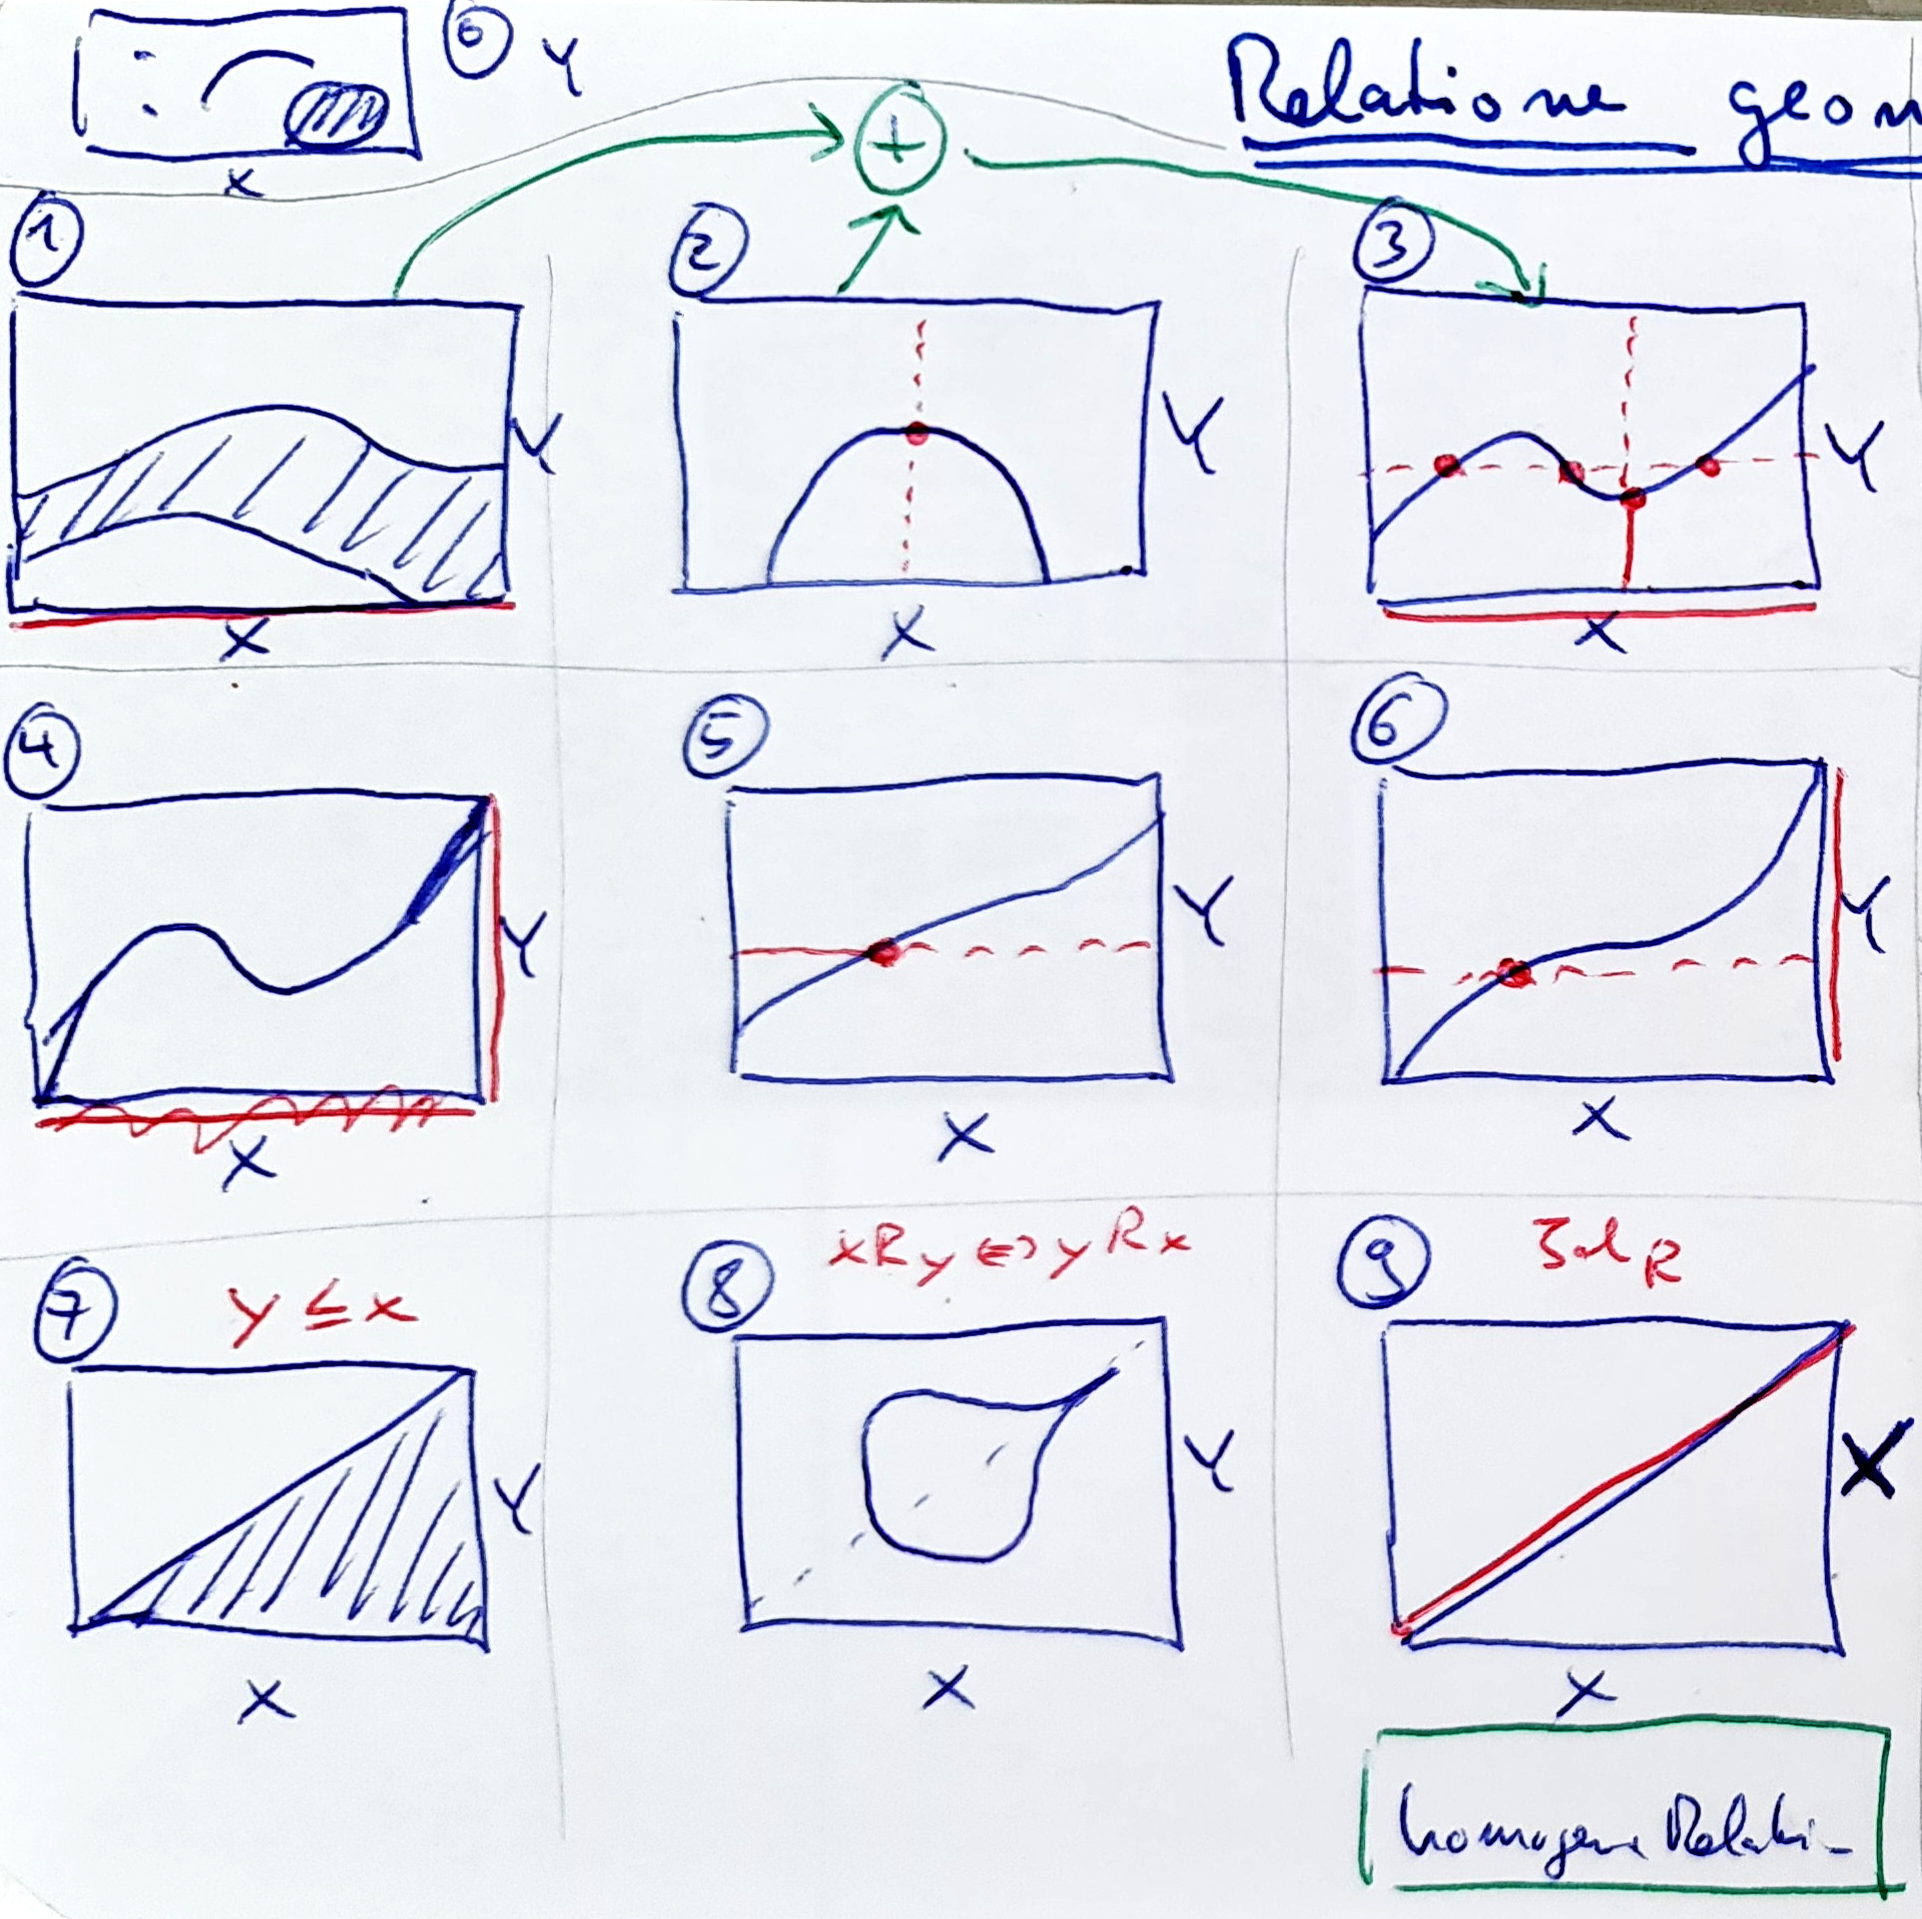
\includegraphics{v3.0.2.0.2 Relationen und Funktionen - Geometrisches Bild Grafik Links.png}
\end{figure}

\begin{figure}
   \centering
   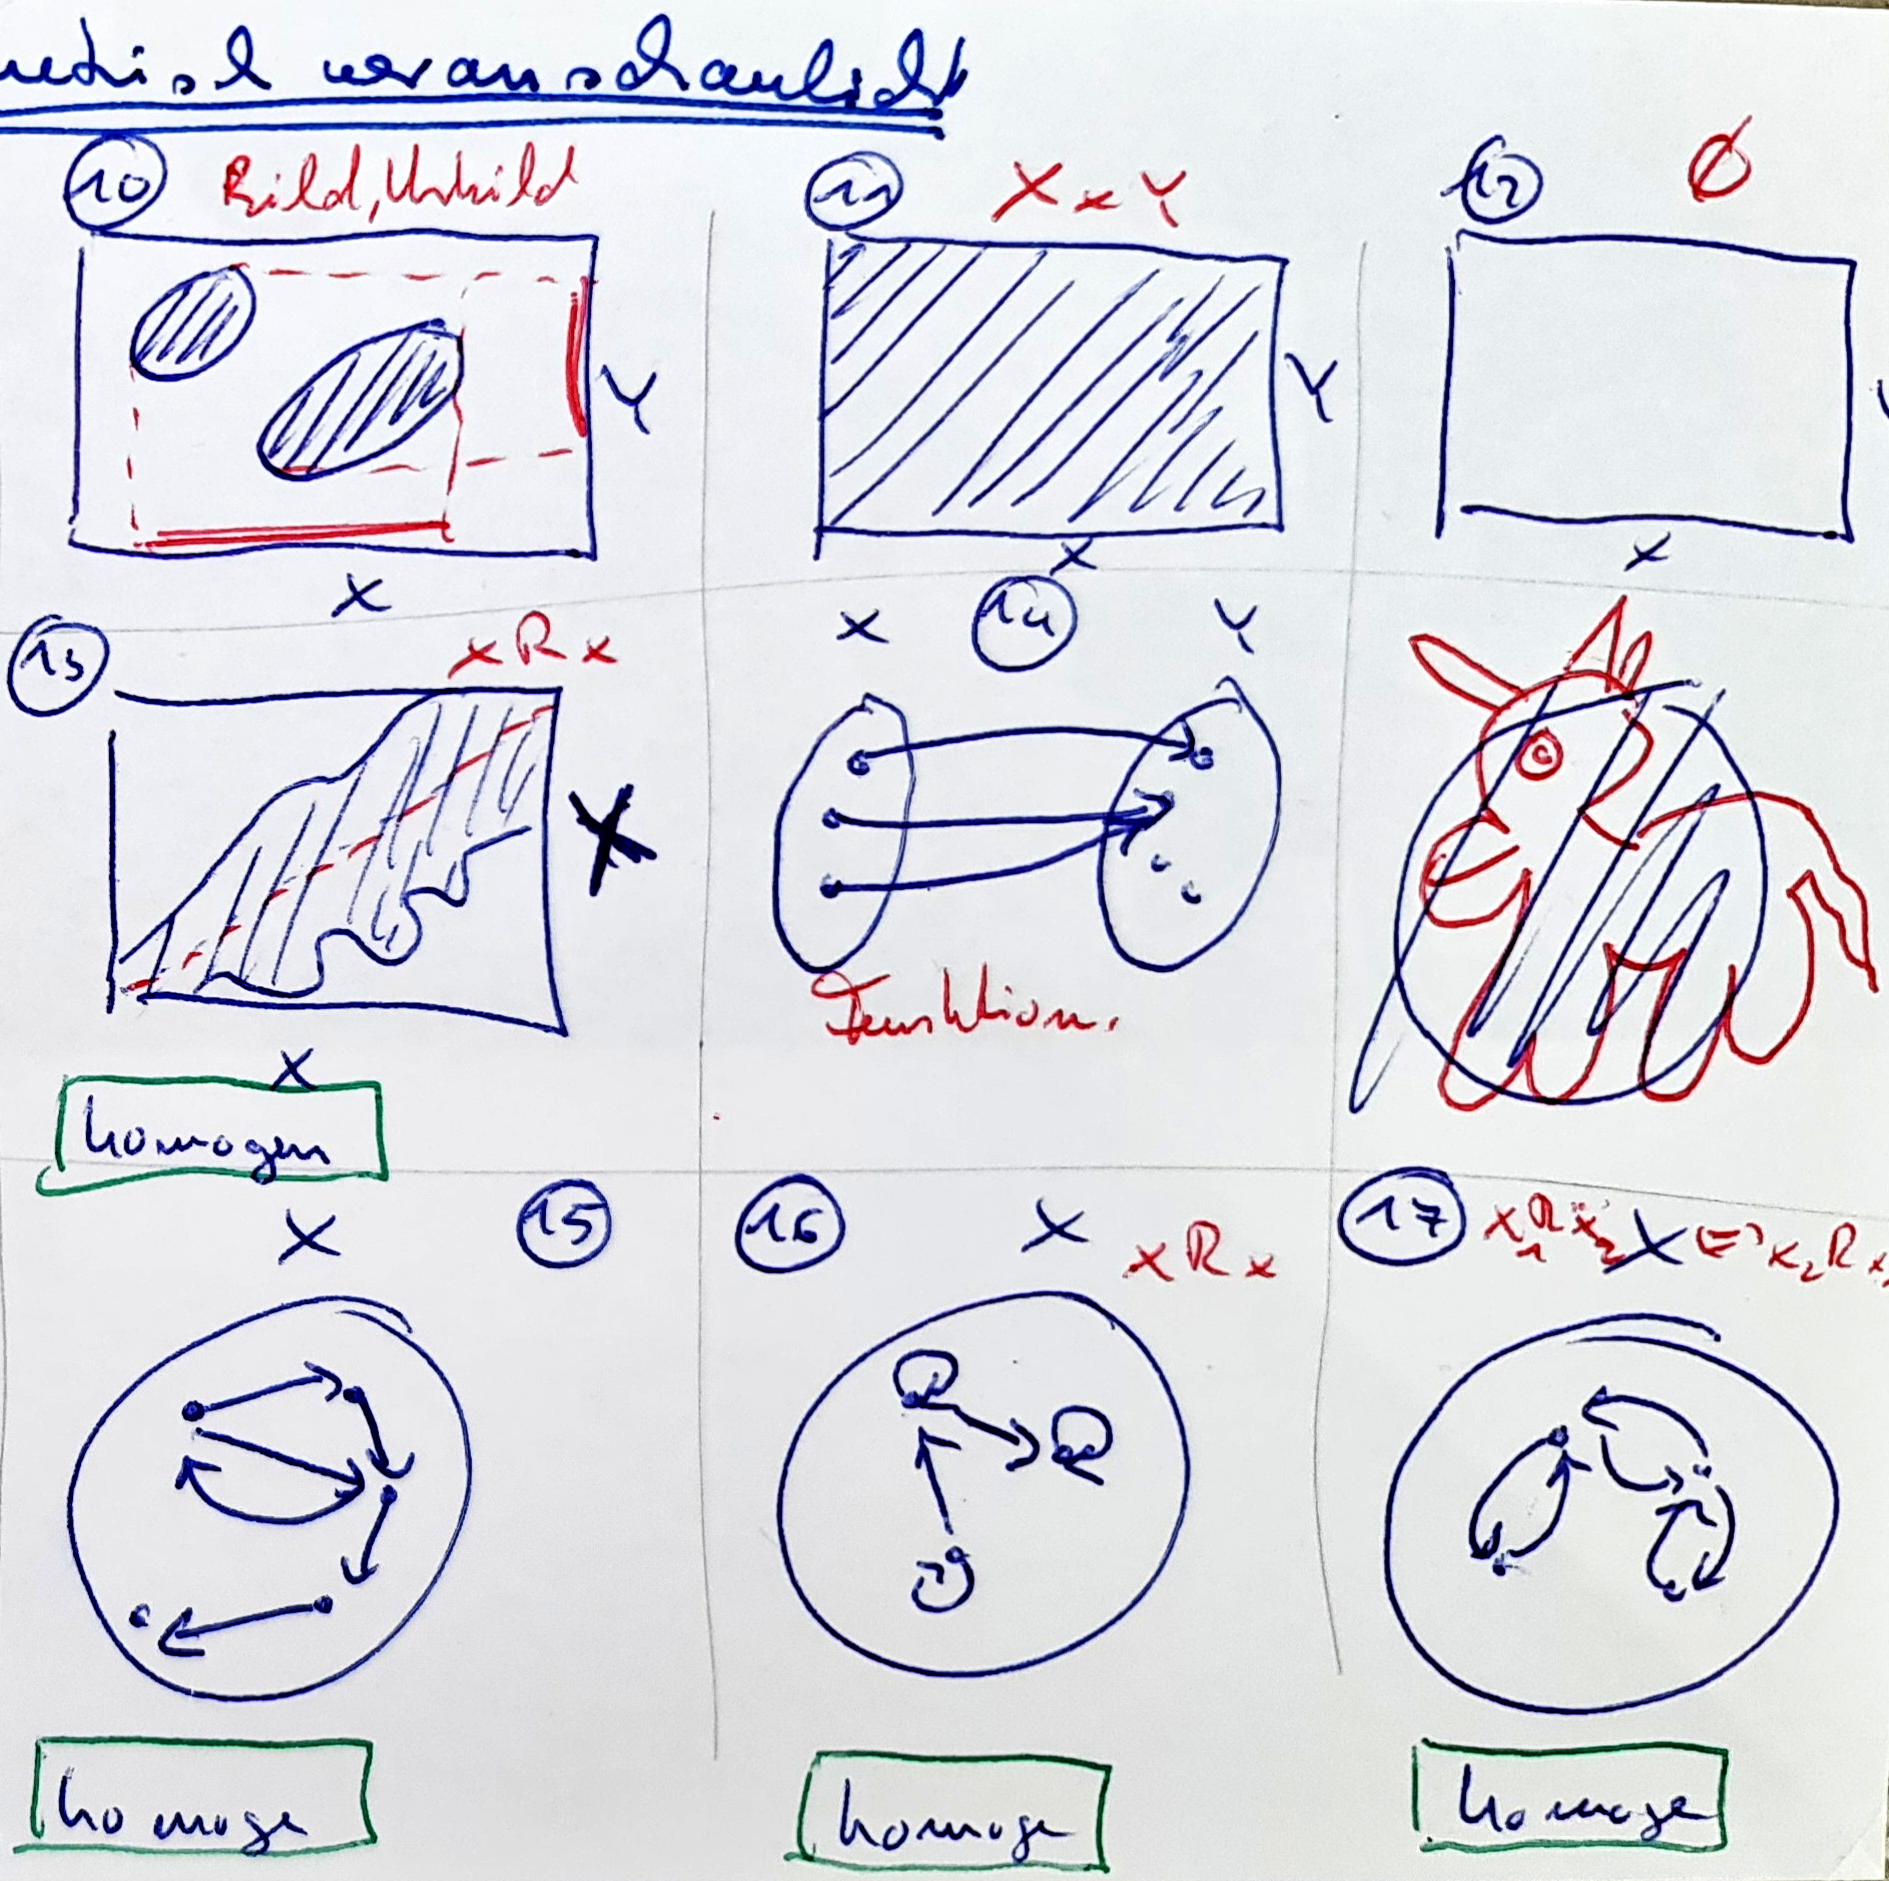
\includegraphics{v3.0.2.0.2 Relationen und Funktionen - Geometrisches Bild Grafik Rechts.png}
\end{figure}

%******************************************************************************************************
%                                                                                                     *
\section{TODO}
%                                                                                                     *
%******************************************************************************************************
\begin{backup}
Noch zu erledigen sind
\begin{itemize}
   \item leer
\end{itemize}
\end{backup}

\begin{backup}
    (Zur Zeit nicht benötigter Inhalt)
\end{backup}

%******************************************************************************************************
%                                                                                                     *
\begin{thebibliography}{9}
%                                                                                                     *
%******************************************************************************************************

   \bibitem[MacLane1978]{MacLane}
      Saunders Mac Lane, \emph{Categories for the Working Mathematician},
      Springer-Verlag New York Inc., 978-0-387-98403-2 (ISBN)
      
   
      
\end{thebibliography}

%******************************************************************************************************
%                                                                                                     *
\begin{large}
    \centerline{\textsc{Symbolverzeichnis}}
\end{large}
%                                                                                                     *
%******************************************************************************************************
\bigskip

\renewcommand*{\arraystretch}{1}

\begin{tabular}{ll}
    $A, B, C, \cdots, X, Y, Z$          & Objekte\\
    $\mathcal F,\mathcal G$             & Funktoren\\
    $f, g, h, r, s, \cdots$             & Homomorphismen\\
   
\end{tabular}

\end{document}
